% PolyForge — defense slides.  Build: pdflatex -interaction=nonstopmode -enable-installer slides.tex
\documentclass[aspectratio=169,11pt]{beamer}

\usetheme{Madrid}
\usecolortheme{dolphin}
\setbeamertemplate{navigation symbols}{}
\usepackage[T1]{fontenc}
\usepackage{lmodern}
\usepackage{booktabs}
\usepackage{graphicx}
\usepackage{amsmath}

\graphicspath{{../../eval/results/figures/}}

\newcommand{\dz}{d_z}

\title{PolyForge: Joint Cross-Layer Control of Replicas,\\
Semantic Cache, and Model Tier for Multi-Tenant Hybrid Serving}
\author{Mohaiminul}
\date{July 2026}

\begin{document}

\maketitle

\begin{frame}{The problem}
  \begin{itemize}
    \item Multi-tenant platforms serve \alert{hybrid} workloads: CRUD $+$ AI
          inference, same tenants, same cluster.
    \item Three control surfaces set cost and quality: \textbf{replica
          autoscaling}, \textbf{semantic caching}, \textbf{model-tier
          routing}.
    \item Today: three independent controllers, each locally optimal, none
          aware of the others --- yet they share one budget, one SLO, one
          tenant set.
  \end{itemize}
  \vfill
  \textbf{Question: do per-layer local optima compose?}
\end{frame}

\begin{frame}{Thesis statement}
  \begin{quote}
    Per-layer local optima do \alert{not} compose. A controller that plans
    replicas, cache budget, and model tier \alert{together} --- one
    receding-horizon optimization against
    $J = \text{cost} + 2\cdot\text{violation} + 0.5\,(1-\text{Jain})$ ---
    dominates tuned per-layer baselines.
  \end{quote}
  \vfill
  Tested under \textbf{7 pre-registered protocols} (pushed before runs),
  \textbf{tuned} baselines, paired seeds, effect sizes with bootstrap CIs
  --- and \textbf{published nulls}.
\end{frame}

\begin{frame}{PolyForge in one loop}
  \begin{itemize}
    \item \textbf{Control plane} (Go): tenants, API keys, RLS-proven
          isolation, telemetry.
    \item \textbf{AI gateway} (Go): routing, semantic cache with cost-aware
          eviction.
    \item \textbf{Classifier}: 12-feature windows $\to$ 5-class taxonomy,
          drift-checked, every 10\,s.
    \item \textbf{JCAC planner}: MPC over a move-blocked lattice
          ($\le 60$ candidates/tenant); the deployed service \alert{imports
          the simulator's controller} --- same code offline and online.
    \item \textbf{Operator}: 4 CRDs; guardrails --- replica bounds, budget
          caps, last-good-plan fallback; shared-target plans are summed, not
          overwritten.
  \end{itemize}
\end{frame}

\begin{frame}{Methodology: the part built to be attacked}
  \begin{itemize}
    \item 7 pre-registrations committed \textbf{and pushed before any run};
          closed campaigns immutable; stopping rules enforced.
    \item Baselines (HPA, KEDA, FIRM, GPTCache-LRU, static, VTC-replica,
          iso-cost) \textbf{grid-tuned on our own objective}.
    \item Paired seeds; citable unit $=$ $\dz$ with 95\% bootstrap CI;
          p-values appear once, as prereg gates.
    \item Substrates never mixed; samples never pooled; p95 not p99
          (documented).
    \item \textbf{Honest-nulls ledger}: 7 published negatives.
  \end{itemize}
\end{frame}

\begin{frame}{Headline matrix: 1{,}800 runs, 500 ablations}
  \centering
  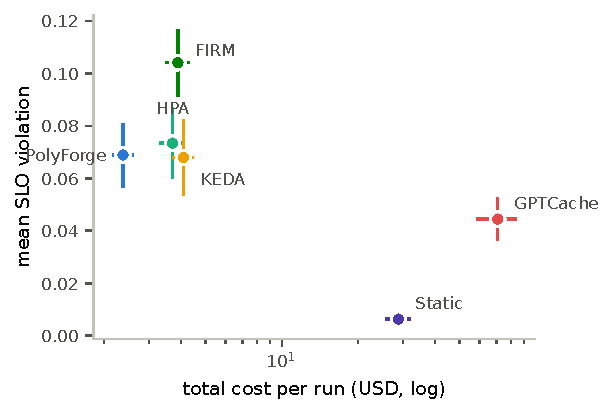
\includegraphics[height=0.62\textheight]{fig03_pareto_cost_violation.pdf}

  \small Wins composite $J$ vs.\ every tuned baseline
  ($|\dz|$ 0.66--1.44); only Pareto-undominated system.
  Ablations: $-$jointness $= +2884\%$ cost.
\end{frame}

\begin{frame}{Joint control, visible in one trace}
  \centering
  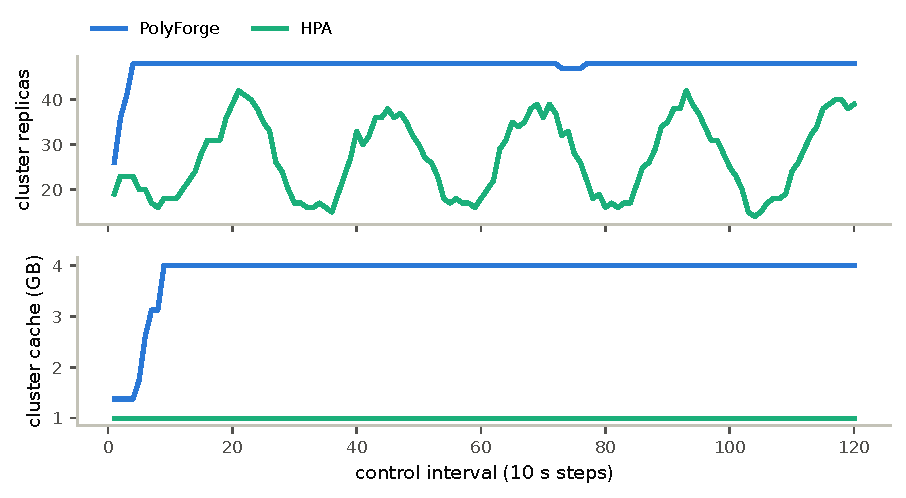
\includegraphics[height=0.68\textheight]{fig09_adaptation_trace.pdf}

  \small First minute of an agentic burst: replicas \emph{and} cache move
  together; HPA has one knob.
\end{frame}

\begin{frame}{Real demand: BurstGPT replays}
  \begin{itemize}
    \item Real trace: 10.63M requests / 335 days, deterministic ETL.
    \item First sample $n{=}16$: \alert{HT FAIL} (underpowered) --- point
          estimates reproduce the v1 ranking. Published as measured.
    \item Powered replay $n{=}96$ (new prereg): \textbf{HT2 PASS} ---
          $J$ beats HPA/KEDA/FIRM ($p \le 5.5{\times}10^{-5}$,
          $\dz$ $-0.43\ldots{-0.47}$),
          \alert{cost $-70\%$} ($p \le 4.3{\times}10^{-6}$),
          violation trade $+0.07$ \textbf{disclosed as pre-registered}.
  \end{itemize}
  \vfill
  \small Cite $-70\%$ ($n{=}96$), never the underpowered sample's $-76\%$.
\end{frame}

\begin{frame}{The SLO story, told honestly}
  \begin{itemize}
    \item v2 H1: beat tuned HPA/KEDA on violation? \alert{FAIL} --- parity,
          at $-43\ldots{-48\%}$ cost.
    \item v3 H1$'$ (overload cells): \alert{FAIL} --- reactive scalers buy
          attainment at \textbf{3.2--3.4$\times$ spend}; only PolyForge
          honors the capacity cap.
    \item v3 H2$'$: seasonal $<$ trend on violation where periodicity
          exists: \textbf{PASS} ($p=6{\times}10^{-4}$, no cost premium).
    \item Spike class (declared exploratory): beats HPA on violation
          \emph{and} cost ($p=5{\times}10^{-5}$, $-46\%$).
    \item Stopping rule: no third confirmatory attempt. The goalposts are in
          the git history.
  \end{itemize}
\end{frame}

\begin{frame}{Forecasting: the data corrected us}
  \centering
  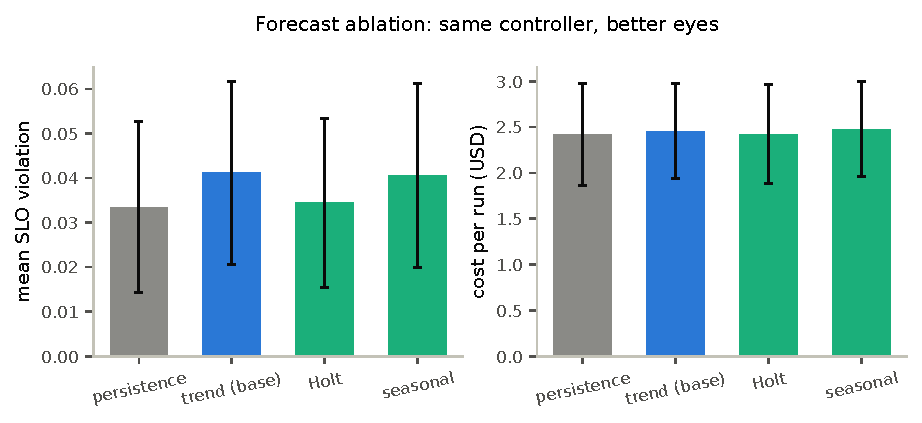
\includegraphics[height=0.5\textheight]{fig13_forecast_ablation.pdf}

  \small Synthetic stand-in predicted seasonal $-44.8\%$ RMSE ---
  \alert{did not transfer} to real BurstGPT (Holt $-26.9\%$ wins).
  Azure LLM 2024 reproduces the boundary: the winner tracks measured
  periodicity $\Rightarrow$ per-tenant, pluggable forecasting.
\end{frame}

\begin{frame}{Semantic cache on real LMSYS-Chat-1M}
  \begin{itemize}
    \item Adaptive hit rate \textbf{29.6\% @ cosine 0.85} (48.8\% @ 0.70);
          $+93\%$ vs.\ a 10\%-fixed cache; \$0.296/1k queries.
    \item Empirical $h(K)$: $h_{\max}{=}0.285$, $K_{1/2}{\approx}6.6$k
          entries --- sim's curve was optimistic; documented, constants
          untouched.
    \item \textbf{Hit precision measured} (frozen protocol): 0.313 overall
          @ $\tau{=}0.85$; same-model $\approx 2\times$ cross-model;
          near-duplicate ceiling 0.338 $\Rightarrow$ cite the shape, not the
          absolute.
  \end{itemize}
\end{frame}

\begin{frame}{Fairness and security}
  \begin{columns}
    \begin{column}{0.52\textwidth}
      \small\textbf{Fairness (control-plane altitude)}
      \begin{itemize}\small
        \item vs.\ FIRM: Jain 0.9689 / 0.9294 ($\dz{=}1.0$).
        \item vs.\ tuned VTC-replica: wins $J$ ($\dz{=}{-1.12}$) \emph{and
              Jain itself} (0.9705 / 0.9599) at $-35\%$ cost.
        \item Own $\gamma$-term: \alert{published null}.
      \end{itemize}
    \end{column}
    \begin{column}{0.44\textwidth}
      \small\textbf{Security}
      \begin{itemize}\small
        \item Shared cache leaks membership: AUC \textbf{0.88} from timing
              alone.
        \item Per-tenant partitioning $\to$ chance (0.50) at 24\% latency
              cost, 76\% hits kept --- dominates padding \& TTL jitter.
      \end{itemize}
    \end{column}
  \end{columns}
  \vspace{2mm}
  \centering
  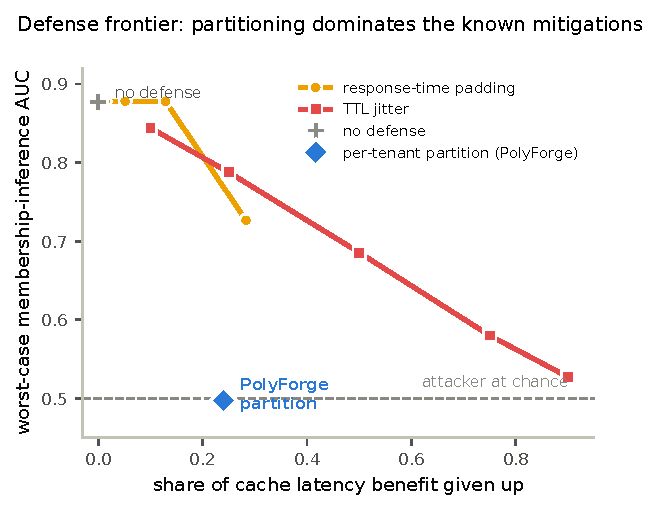
\includegraphics[height=0.36\textheight]{fig17_defense_frontier.pdf}
\end{frame}

\begin{frame}{Theory, at the code's altitude}
  \begin{itemize}
    \item \textbf{Prop.\ 1}: the two-sweep solver returns a
          block-coordinate minimum of $J$ --- no tenant improves
          unilaterally. (Not claimed: global optimality; Jain coupling is
          non-separable.)
    \item \textbf{Prop.\ 2}: self-calibration scale is confined to
          $[0.5,1]$, only ever conservative, and returns to full trust in
          $\le 25$ agreeing steps --- safety independent of tuning.
    \item Measured scale: planner growth exponent \textbf{1.45}; 3\,s
          timeout crossed at 128 tenants; past it, designed fallback.
  \end{itemize}
\end{frame}

\begin{frame}{Validity: what bounds the simulator gap}
  \begin{itemize}
    \item \textbf{Calibration errs against us}: congestion fit $a{=}0.86$
          vs.\ assumed 1.0; GPU tier bench confirms ordering (1:1.5:16.6).
    \item \textbf{Real data carries the claims}: BurstGPT $+$ Azure demand,
          LMSYS prompts.
    \item \textbf{Live check is ordinal-only}: HPA arm verified on a real
          kind cluster; JCAC arm fully wired, gated by an executable
          actuation check; analysis protocol $+$ figure caption frozen
          \emph{before} any live number exists.
  \end{itemize}
  \vfill
  Not claimed: absolute dollars/latency on production fleets; token-level
  fairness; p99 on sim.
\end{frame}

\begin{frame}{Contributions}
  \begin{enumerate}
    \item First joint replicas$+$cache$+$tier controller with per-tenant
          dollar accounting.
    \item The composition gap, measured: $+2884\%$ cost without jointness;
          $-70\%$ cost on real demand vs.\ tuned scalers.
    \item Honest SLO account: parity at $-43\ldots{-48\%}$ cost; mechanism
          confirmed; two failures published.
    \item Real-data cache results \emph{with a quality denominator}.
    \item Fairness wins at stated altitude; own term nulled in public.
    \item Cache side-channel attack $+$ dominant defense frontier.
    \item Two construction-level solver guarantees.
    \item A pre-registered, null-publishing systems methodology --- in git,
          diffable.
  \end{enumerate}
\end{frame}

\begin{frame}{What remains, and closing}
  \textbf{Remaining measurement (one Docker sitting):} the live JCAC ordinal
  slice --- protocol, caption, and honesty gate already frozen; reported
  ordinal-only whichever way it lands.
  \vfill
  \textbf{Future work:} token-level demand signals (llm-d/AIBrix
  substrate), p99 live restatement, planner scaling past 128 tenants,
  pre-registered adoption of the empirical cache curve.
  \vfill
  \begin{quote}
    The strongest sentence in this thesis is not a percentage --- it is
    that every percentage traces to a protocol committed before the run.
  \end{quote}
\end{frame}

\end{document}
